%%%%%%%%%%%%%%%%%%%%%%%%%%%%%%%%%%%%%%%%%
% Short Sectioned Assignment LaTeX Template Version 1.0 (5/5/12)
% This template has been downloaded from: http://www.LaTeXTemplates.com
% Original author:  Frits Wenneker (http://www.howtotex.com)
% License: CC BY-NC-SA 3.0 (http://creativecommons.org/licenses/by-nc-sa/3.0/)
%%%%%%%%%%%%%%%%%%%%%%%%%%%%%%%%%%%%%%%%%

%----------------------------------------------------------------------------------------
%	PACKAGES AND OTHER DOCUMENT CONFIGURATIONS
%----------------------------------------------------------------------------------------

\documentclass[paper=a4, fontsize=11pt]{scrartcl} % A4 paper and 11pt font size

% ---- Entrada y salida de texto -----

\usepackage[T1]{fontenc} % Use 8-bit encoding that has 256 glyphs
\usepackage[utf8]{inputenc}
%\usepackage{fourier} % Use the Adobe Utopia font for the document - comment this line to return to the LaTeX default

% ---- Idioma --------

\usepackage[spanish, es-tabla]{babel} % Selecciona el español para palabras introducidas automáticamente, p.ej. "septiembre" en la fecha y especifica que se use la palabra Tabla en vez de Cuadro

% ---- Otros paquetes ----

\usepackage{url} % ,href} %para incluir URLs e hipervínculos dentro del texto (aunque hay que instalar href)
\usepackage{amsmath,amsfonts,amsthm} % Math packages
%\usepackage{graphics,graphicx, floatrow} %para incluir imágenes y notas en las imágenes
\usepackage{graphics,graphicx, float} %para incluir imágenes y colocarlas
% Para hacer cuadros
\usepackage{tcolorbox}
% Para hacer uso de párrafos
\usepackage{parskip}
\usepackage{hyperref}
\usepackage{vmargin}
\setpapersize{A4}
\setmargins{2.5cm}       % margen izquierdo
{1.5cm}                        % margen superior
{16.5cm}                      % anchura del texto
{23.42cm}                    % altura del texto
{10pt}                           % altura de los encabezados
{1cm}                           % espacio entre el texto y los encabezados
{0pt}                             % altura del pie de página
{2cm}                           % espacio entre el texto y el pie de página
% Para hacer tablas comlejas
%\usepackage{multirow}
%\usepackage{threeparttable}

%\usepackage{sectsty} % Allows customizing section commands
%\allsectionsfont{\centering \normalfont\scshape} % Make all sections centered, the default font and small caps

\usepackage{fancyhdr} % Custom headers and footers
\pagestyle{fancyplain} % Makes all pages in the document conform to the custom headers and footers
\fancyhead{} % No page header - if you want one, create it in the same way as the footers below
\fancyfoot[L]{Mario López González 3ºB} % Empty left footer
\fancyfoot[C]{} % Empty center footer
\fancyfoot[R]{\thepage} % Page numbering for right footer
\renewcommand{\headrulewidth}{0pt} % Remove header underlines
\renewcommand{\footrulewidth}{0pt} % Remove footer underlines
\setlength{\headheight}{13.6pt} % Customize the height of the header

\numberwithin{equation}{section} % Number equations within sections (i.e. 1.1, 1.2, 2.1, 2.2 instead of 1, 2, 3, 4)
\numberwithin{figure}{section} % Number figures within sections (i.e. 1.1, 1.2, 2.1, 2.2 instead of 1, 2, 3, 4)
\numberwithin{table}{section} % Number tables within sections (i.e. 1.1, 1.2, 2.1, 2.2 instead of 1, 2, 3, 4)

\setlength\parindent{0pt} % Removes all indentation from paragraphs - comment this line for an assignment with lots of text

\newcommand{\horrule}[1]{\rule{\linewidth}{#1}} % Create horizontal rule command with 1 argument of height


\title{	
\normalfont \normalsize 
\textsc{\textbf{Ingeniería de Servidores (2021-2022)} \\ Grado en Ingeniería Informática \\ Universidad de Granada} \\ [25pt] % Your university, school and/or department name(s)
\horrule{0.5pt} \\[0.4cm] % Thin top horizontal rule
\huge Memoria Práctica 3 \\ % The assignment title
\horrule{2pt} \\[0.5cm] % Thick bottom horizontal rule
}

\author{Mario López González} % Nombre y apellidos

\date{\normalsize\today} % Incluye la fecha actual

%----------------------------------------------------------------------------------------
% DOCUMENTO
%----------------------------------------------------------------------------------------

\begin{document}

\maketitle % Muestra el Título

\newpage %inserta un salto de página

\tableofcontents % para generar el índice de contenidos
\listoffigures % para generar el índice de imágenes

\newpage
%----------------------------------------------------------------------------------------
%	Cuestión 1
%----------------------------------------------------------------------------------------

% \section{Instalación de Zabbix}

% \begin{tcolorbox}[colback=black!10, halign=left]
% \$ sudo apt update
% \\ \$ sudo apt update
% \end{tcolorbox}

% \begin{figure}[H]
%     \centering
%     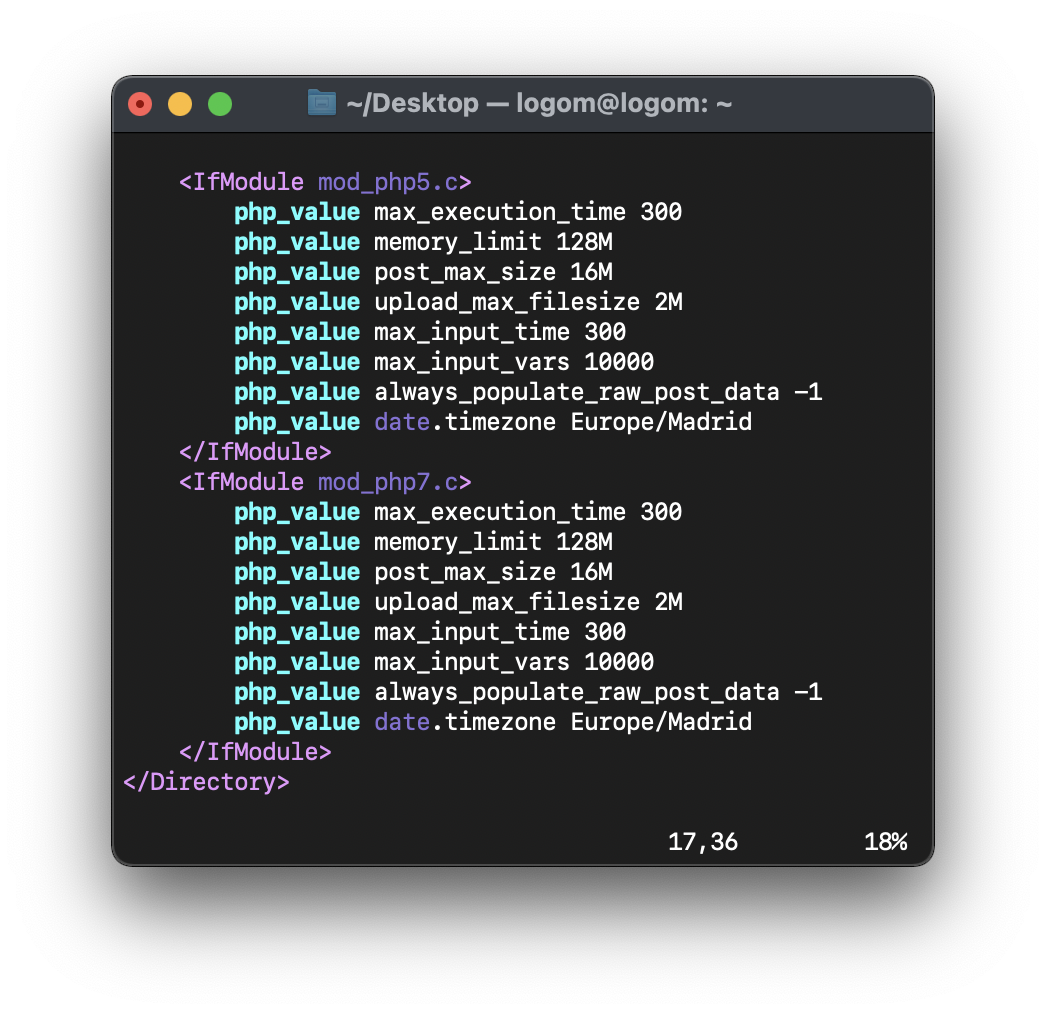
\includegraphics[scale=0.75]{images/apache_conf.png}
%     \caption{titulo de la foto}
%     \label{fig:id}
% \end{figure}

\section{Ejercicio 1}
\subsection{Descargar paquetes de Zabbix 5.0}

    Vamos a descargar los paquetes de Zabbix, para ello entramos en su web oficial, \href{https://www.zabbix.com/download}{Zabbix.com}, y 
    seleccionamos los siguientes parámetros ya que son los que se ajustan a nuestras necesidades.
        
    \begin{figure}[H]
        \centering
        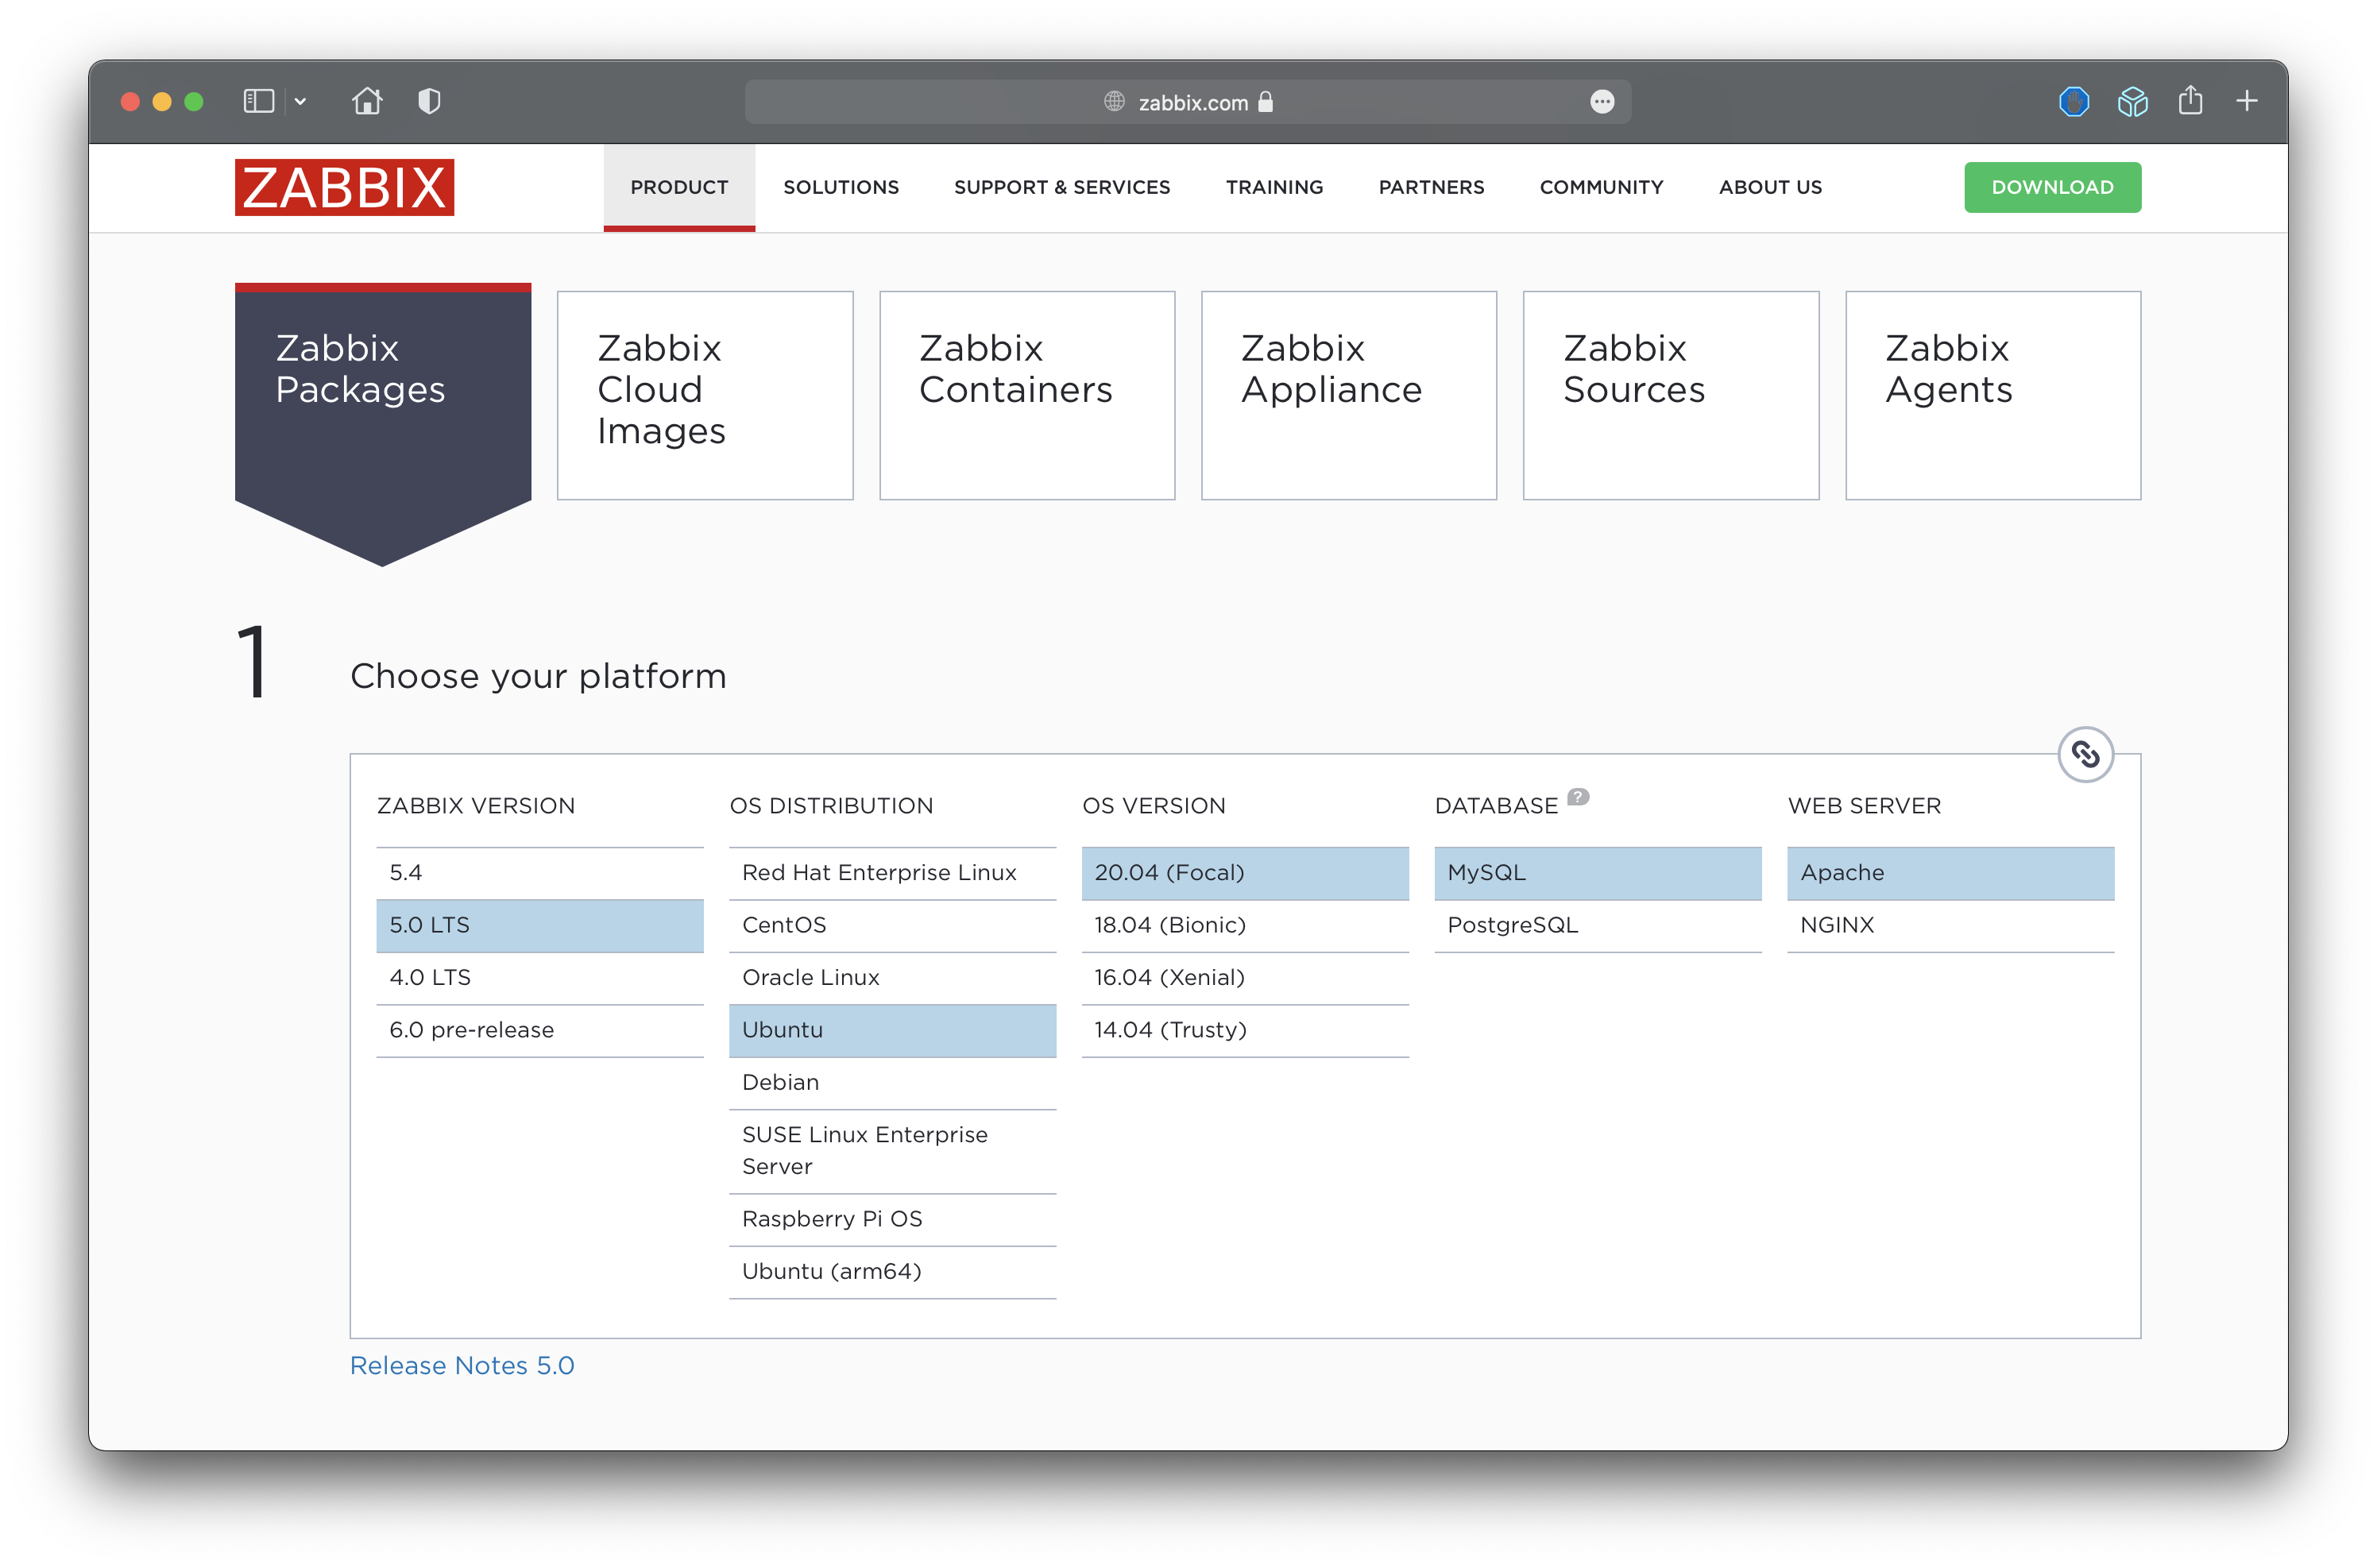
\includegraphics[scale=0.3]{images/zabbix_official.png}
        \caption{Descargar Zabbix desde paquetes}
        \label{fig:zabbix_official}
    \end{figure}

    Lo primero que debemos hacer es descargar los paquetes correspondientes a Zabbix 5.0 desde su repositorio oficial con el comando \textbf{\emph{wget}}. 
        \begin{tcolorbox}[colback=black!10, halign=left]
            \$ wget https://repo.zabbix.com/zabbix/5.0/ubuntu/pool/main/z/zabbix-release/zabbix-release\_5.0-1+focal\_all.deb
        \end{tcolorbox}

    Una vez descargado, lo instalamos el repositorio con el comando \textbf{\emph{dpkg}}.
        \begin{tcolorbox}[colback=black!10, halign=left]
            \$ sudo dpkg -i zabbix-release\_5.0-1+focal\_all.deb
        \end{tcolorbox}

    Por último actualizamos la lista de paquetes disponibles y sus versiones.
        \begin{tcolorbox}[colback=black!10, halign=left]
            \$ sudo apt update
        \end{tcolorbox}

    \newpage
    \subsection{Instalar Zabbix}

    Ya tenemos todos los paquetes descargados y actualizados, por lo tanto, lo siquiente que indica la web es que hay que instalar Zabbix server, frontend
    y agent con el comando \textbf{\emph{apt install}}.
        \begin{tcolorbox}[colback=black!10, halign=left]
            \$ sudo apt install zabbix-server-mysql zabbix-frontend-php zabbix-apache-conf zabbix-agent
        \end{tcolorbox}
    
    \subsection{Crear base de datos inicial}
    Antes de crear la base de datos inicial debemos estar seguros de que el sistema está encendido y funcionando. Una vez hechas las comprobaciones previas,
    pasamos a crear la base de datos. Para ello ingresamos en el asistente de mysql.
        \begin{tcolorbox}[colback=black!10, halign=left]
            \$ sudo mysql -u root -p

            \emph{Ingresamos la contraseña para ingresar en la base de datos (ISE)}
        \end{tcolorbox}

    Una vez dentro del asistente ejecutamos los siguientes comandos en PostgreSQL:
        \begin{tcolorbox}[colback=black!10, halign=left]
            mysql> create database zabbix character set utf8 collate utf8\_bin;

            mysql> create user zabbix@localhost identified by 'ISE';

            mysql> grant all privileges on zabbix.* to zabbix@localhost;

            mysql> quit;
        \end{tcolorbox}

    Definimos la nueva contraseña creada con el siguiente comando y escribimos la contraseña.
        \begin{tcolorbox}[colback=black!10, halign=left]
            \$ sudo zcat /usr/share/doc/zabbix-server-mysql*/create.sql.gz | mysql -uzabbix -p zabbix
            \emph{Ingresamos la contraseña (ISE)}
        \end{tcolorbox}

    \subsection{Configurar la base de datos de Zabbix server}
    Editamos el fichero que se encuentra en la siguiente ruta /etc/zabbix/zabbix\_server.conf, descomentamos el parámetro \textbf{\emph{DBPassword}} y le asignamos el valor
    \textbf{\emph{ISE}}:
    \begin{figure}[H]
        \centering
        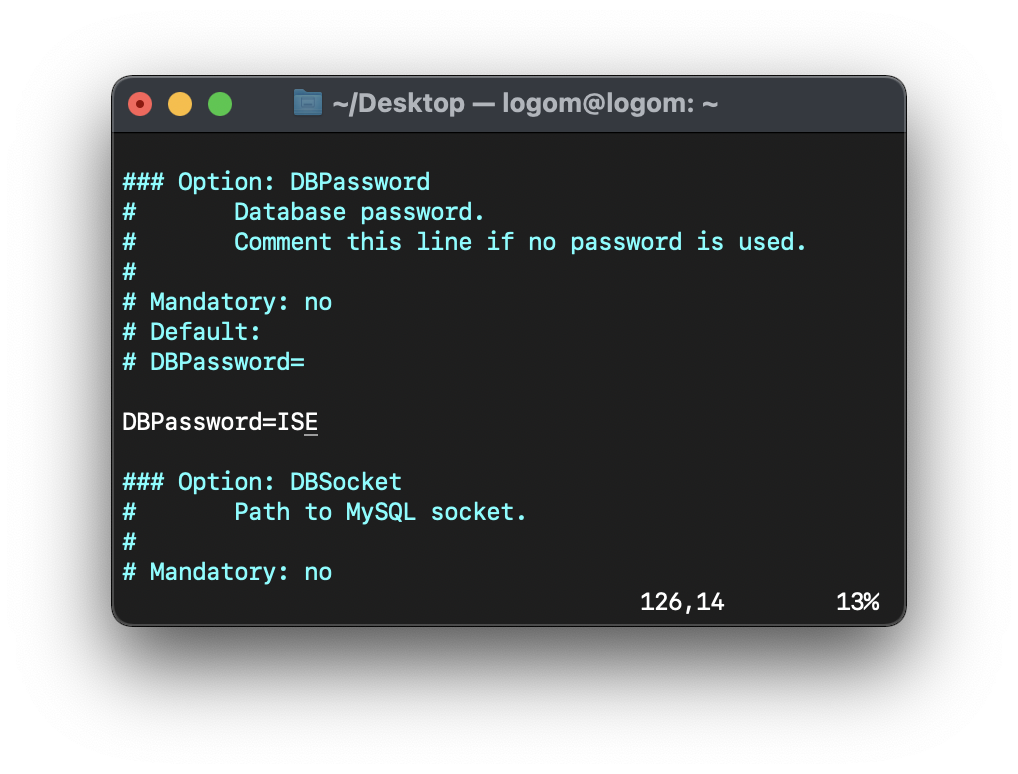
\includegraphics[scale=0.4]{images/zabbix_server_conf.png}
        \caption{Configuración base de datos}
        \label{fig:zabbix_conf}
    \end{figure}

    \subsection{Configurar el PHP del frontend de Zabbix}
    Editamos el fichero que se encuentra en la siguiente ruta /etc/zabbix/apache.conf y modificamos el parámetro comentado \textbf{\emph{php\_value date.timezone}} reemplazando Riga
    por Madrid para que se muestre la hora de forma correcta.
    \begin{figure}[H]
        \centering
        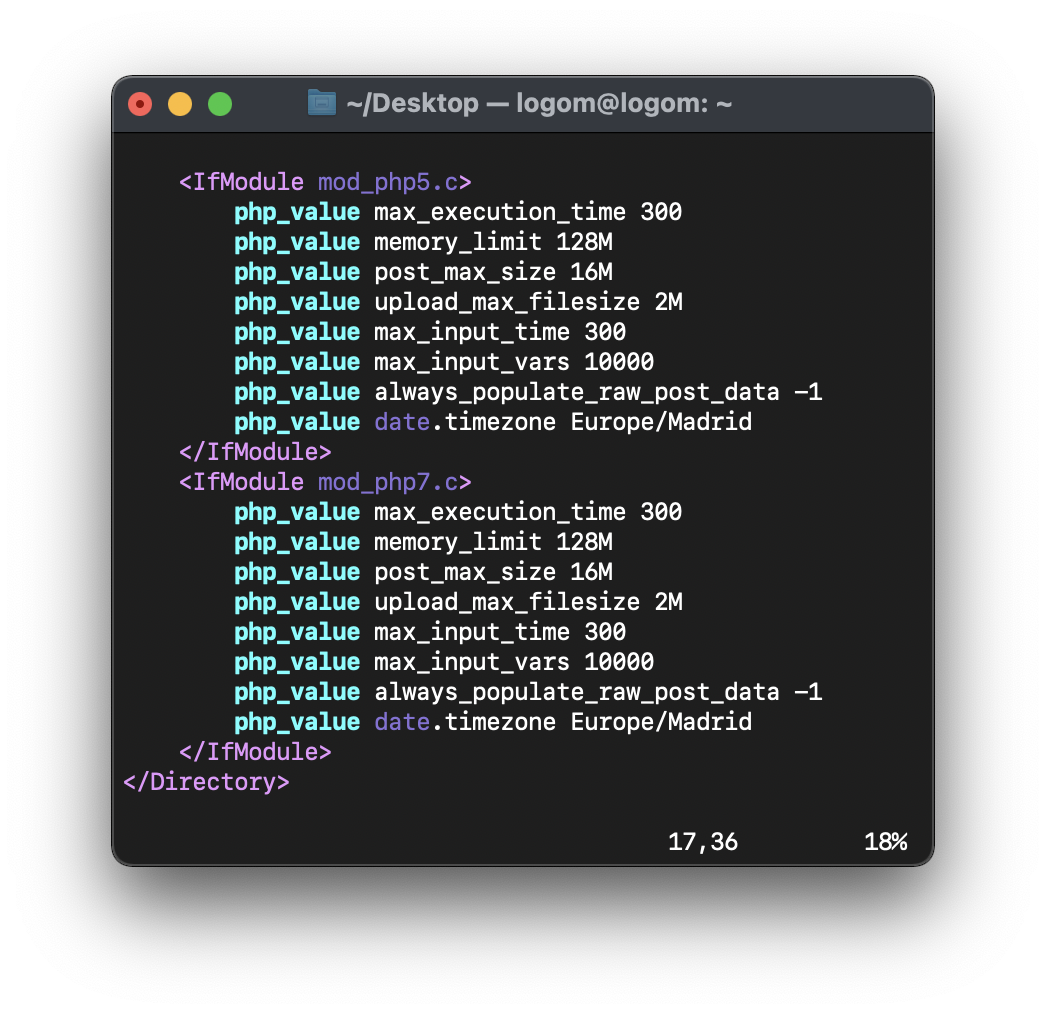
\includegraphics[scale=0.5]{images/apache_conf.png}
        \caption{Configuración base de datos}
        \label{fig:apache_conf}
    \end{figure}

    \subsection{Configurar los servicios}
    Reiniciamos los servicios zabbix-server, zabbix-agent y apache2 para que se actualicen los cambios realizados.
        \begin{tcolorbox}[colback=black!10, halign=left]
            \$ sudo systemctl restart zabbix-server zabbix-agent apache2
        \end{tcolorbox}

    Habilitamos los servicios anteriores para que se enciendan cuando arranque el sistema.
        \begin{tcolorbox}[colback=black!10, halign=left]
            \$ sudo systemctl enable zabbix-server zabbix-agent apache2
        \end{tcolorbox}

    \subsection{Configurar el frontend de Zabbix}

\end{document}
